\documentclass[11pt,a4paper]{article}
\usepackage[utf8]{inputenc}
\usepackage[T1]{fontenc}
\usepackage{graphicx}
\usepackage{float}  % For better figure control with [H] option
\usepackage{tikz}   % For creating diagrams
\usetikzlibrary{shapes.geometric}
\usepackage{pgfplots}
\usepackage{amsmath}
\usepackage{amsfonts}
\usepackage{geometry}
\usepackage{hyperref}
\usepackage{booktabs}
\usepackage{longtable}

% Configure page geometry
\geometry{
    left=2.5cm,
    right=2.5cm,
    top=2.5cm,
    bottom=2.5cm
}

% Configure hyperref
\hypersetup{
    colorlinks=true,
    linkcolor=blue,
    filecolor=magenta,      
    urlcolor=cyan,
    pdftitle={Ziplink System Design},
    pdfauthor={Ziplink Team},
    pdfsubject={URL Shortener System Architecture}
}

\title{Ziplink System Design \\ URL Shortener Architecture}
\author{Ziplink Development Team}
\date{\today}

\begin{document}

\maketitle
\tableofcontents
\newpage

\section{Introduction}

Ziplink is a modern URL shortener web application designed to convert long, unwieldy URLs into short, manageable links that are easy to share and remember. This document outlines the system architecture, design decisions, and implementation details of the Ziplink application.

The system follows a modern three-tier architecture with a React frontend, Node.js/Express backend, and MongoDB database. This design ensures scalability, maintainability, and optimal user experience.

\section{System Architecture Overview}

The Ziplink system architecture is designed with modularity and scalability in mind. Figure~\ref{fig:system-overview} presents the high-level system architecture, showing the interaction between different components.

\begin{figure}[!ht]
\centering
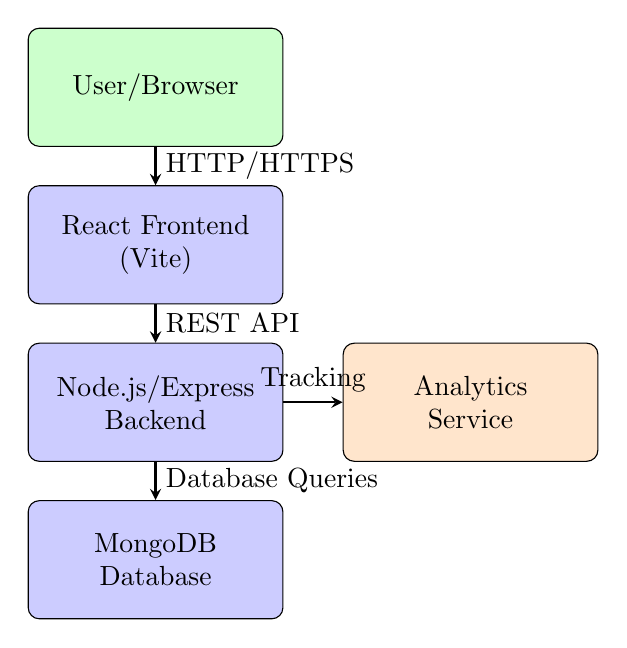
\begin{tikzpicture}[
    node distance=2cm,
    box/.style={rectangle, draw, fill=blue!20, text width=3cm, text centered, rounded corners, minimum height=1.5cm, align=center},
    arrow/.style={->, >=stealth, thick}
]

% User/Client layer
\node[box, fill=green!20] (user) {User/Browser};

% Frontend layer
\node[box, below of=user] (frontend) {React Frontend \\ (Vite)};

% Backend layer
\node[box, below of=frontend] (backend) {Node.js/Express \\ Backend};

% Database layer
\node[box, below of=backend] (database) {MongoDB \\ Database};

% External services
\node[box, right of=backend, xshift=2cm, fill=orange!20] (analytics) {Analytics \\ Service};

% Arrows
\draw[arrow] (user) -- (frontend) node[midway, right] {HTTP/HTTPS};
\draw[arrow] (frontend) -- (backend) node[midway, right] {REST API};
\draw[arrow] (backend) -- (database) node[midway, right] {Database Queries};
\draw[arrow] (backend) -- (analytics) node[midway, above] {Tracking};

\end{tikzpicture}
\caption{High-level system architecture showing the main components and their interactions}
\label{fig:system-overview}
\end{figure}

As illustrated in Figure~\ref{fig:system-overview}, the system consists of four main layers:

\begin{itemize}
    \item \textbf{Presentation Layer}: React-based frontend built with Vite for fast development and optimized builds
    \item \textbf{Application Layer}: Node.js/Express backend handling business logic and API endpoints
    \item \textbf{Data Layer}: MongoDB database for persistent storage of URLs and analytics
    \item \textbf{External Services}: Analytics and monitoring services for tracking URL usage
\end{itemize}

\section{Frontend Architecture}

The frontend is built using React with modern development practices. The component architecture follows a hierarchical structure as shown in Figure~\ref{fig:frontend-architecture}.

\begin{figure}[!htbp]
\centering
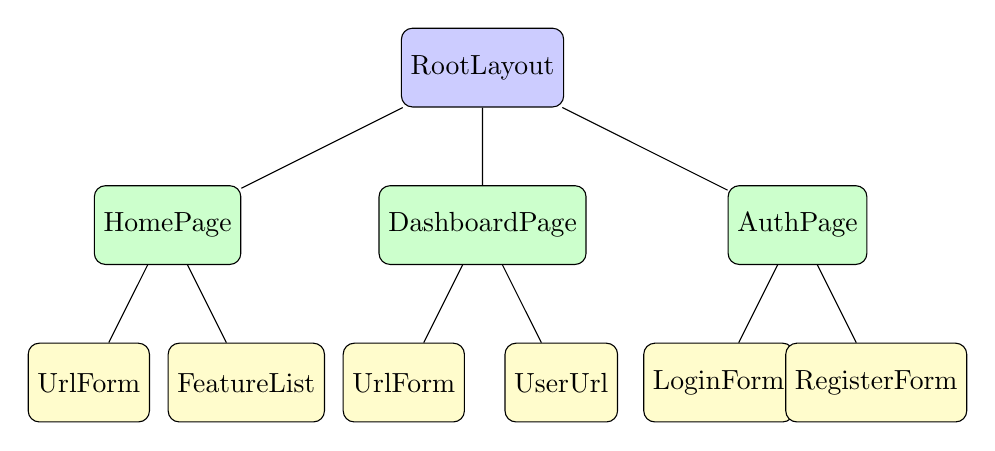
\begin{tikzpicture}[
    level distance=2cm,
    level 1/.style={sibling distance=4cm},
    level 2/.style={sibling distance=2cm},
    every node/.style={rectangle, draw, text centered, rounded corners, minimum height=1cm}
]

\node[fill=blue!20] {RootLayout}
    child {node[fill=green!20] {HomePage}
        child {node[fill=yellow!20] {UrlForm}}
        child {node[fill=yellow!20] {FeatureList}}
    }
    child {node[fill=green!20] {DashboardPage}
        child {node[fill=yellow!20] {UrlForm}}
        child {node[fill=yellow!20] {UserUrl}}
    }
    child {node[fill=green!20] {AuthPage}
        child {node[fill=yellow!20] {LoginForm}}
        child {node[fill=yellow!20] {RegisterForm}}
    };

\end{tikzpicture}
\caption{Frontend component hierarchy showing the main pages and their child components}
\label{fig:frontend-architecture}
\end{figure}

The frontend architecture shown in Figure~\ref{fig:frontend-architecture} implements a clear separation of concerns with:

\begin{itemize}
    \item \textbf{RootLayout}: Main layout component with navigation
    \item \textbf{Page Components}: Route-level components for different application views
    \item \textbf{Feature Components}: Reusable components for specific functionality
\end{itemize}

\section{Backend API Design}

The backend API follows RESTful principles and provides endpoints for URL management and analytics. The API structure is illustrated in Figure~\ref{fig:api-structure}.

\begin{figure}[!ht]
\centering
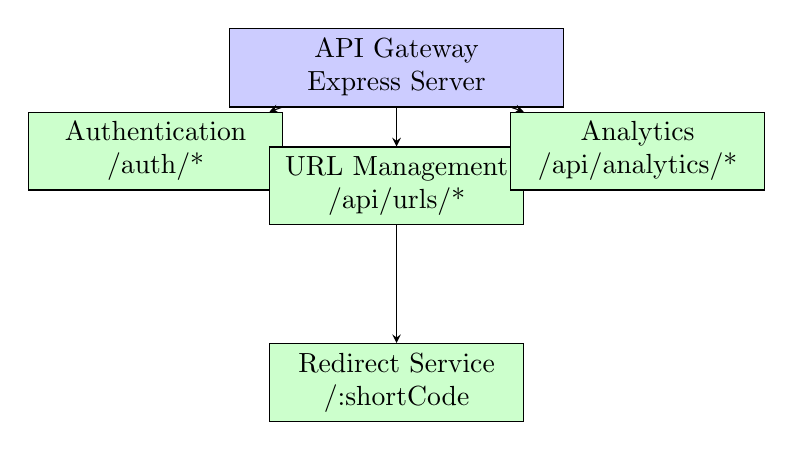
\begin{tikzpicture}[
    node distance=1.5cm,
    api/.style={rectangle, draw, fill=blue!20, text width=4cm, text centered, minimum height=1cm},
    endpoint/.style={rectangle, draw, fill=green!20, text width=3cm, text centered, minimum height=0.8cm}
]

% API Gateway
\node[api] (gateway) {API Gateway\\Express Server};

% Authentication
\node[endpoint, below left of=gateway, xshift=-2cm] (auth) {Authentication\\/auth/*};

% URL Management
\node[endpoint, below of=gateway] (urls) {URL Management\\/api/urls/*};

% Analytics
\node[endpoint, below right of=gateway, xshift=2cm] (analytics) {Analytics\\/api/analytics/*};

% Redirect Service
\node[endpoint, below of=urls, yshift=-1cm] (redirect) {Redirect Service\\/:shortCode};

% Arrows
\draw[->, >=stealth] (gateway) -- (auth);
\draw[->, >=stealth] (gateway) -- (urls);
\draw[->, >=stealth] (gateway) -- (analytics);
\draw[->, >=stealth] (urls) -- (redirect);

\end{tikzpicture}
\caption{Backend API structure showing main service endpoints and their relationships}
\label{fig:api-structure}
\end{figure}

The API structure in Figure~\ref{fig:api-structure} provides clear separation between different service concerns, enabling modular development and easy maintenance.

\section{Database Schema}

The MongoDB database schema is designed to efficiently store URL mappings and analytics data. Figure~\ref{fig:database-schema} shows the main collections and their relationships.

\begin{figure}[!htbp]
\centering
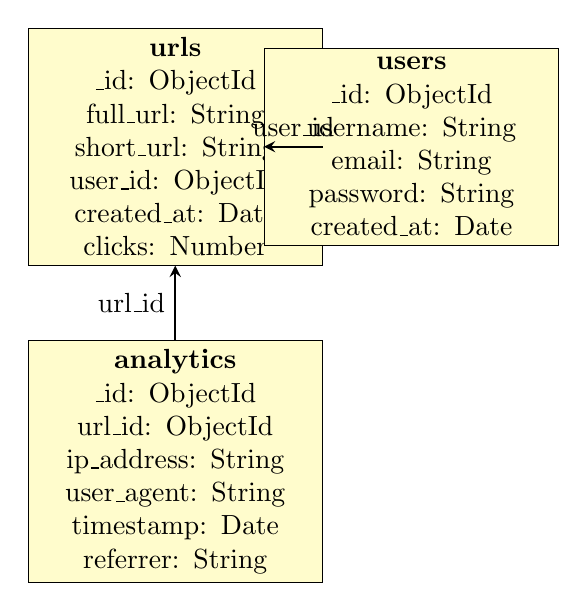
\begin{tikzpicture}[
    node distance=3cm,
    collection/.style={rectangle, draw, fill=yellow!20, text width=3.5cm, text centered, minimum height=2cm}
]

% Collections
\node[collection] (urls) {
    \textbf{urls}\\
    \_id: ObjectId\\
    full\_url: String\\
    short\_url: String\\
    user\_id: ObjectId\\
    created\_at: Date\\
    clicks: Number
};

\node[collection, right of=urls] (users) {
    \textbf{users}\\
    \_id: ObjectId\\
    username: String\\
    email: String\\
    password: String\\
    created\_at: Date
};

\node[collection, below of=urls, yshift=-1cm] (analytics) {
    \textbf{analytics}\\
    \_id: ObjectId\\
    url\_id: ObjectId\\
    ip\_address: String\\
    user\_agent: String\\
    timestamp: Date\\
    referrer: String
};

% Relationships
\draw[->, >=stealth, thick] (urls) -- (users) node[midway, above] {user\_id};
\draw[->, >=stealth, thick] (analytics) -- (urls) node[midway, left] {url\_id};

\end{tikzpicture}
\caption{Database schema showing main collections and their relationships}
\label{fig:database-schema}
\end{figure}

The database schema illustrated in Figure~\ref{fig:database-schema} ensures data integrity and supports efficient queries for both URL operations and analytics reporting.

\section{URL Shortening Algorithm}

The URL shortening process follows a systematic approach to generate unique, short identifiers. The algorithm workflow is depicted in Figure~\ref{fig:shortening-algorithm}.

\begin{figure}[H]
\centering
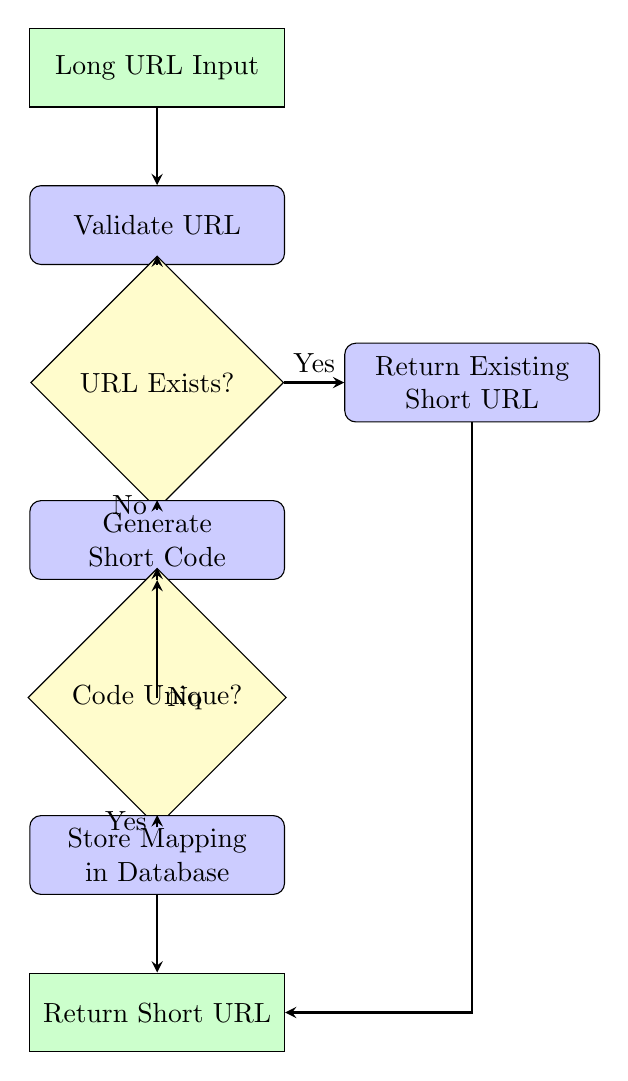
\begin{tikzpicture}[
    node distance=2cm,
    process/.style={rectangle, draw, fill=blue!20, text width=3cm, text centered, rounded corners, minimum height=1cm},
    decision/.style={diamond, draw, fill=yellow!20, text width=2.5cm, text centered, minimum height=1cm},
    data/.style={rectangle, draw, fill=green!20, text width=3cm, text centered, minimum height=1cm},
    arrow/.style={->, >=stealth, thick}
]

\node[data] (input) {Long URL Input};
\node[process, below of=input] (validate) {Validate URL};
\node[decision, below of=validate] (exists) {URL Exists?};
\node[process, right of=exists, xshift=2cm] (return) {Return Existing\\Short URL};
\node[process, below of=exists] (generate) {Generate\\Short Code};
\node[decision, below of=generate] (unique) {Code Unique?};
\node[process, below of=unique] (store) {Store Mapping\\in Database};
\node[data, below of=store] (output) {Return Short URL};

% Arrows
\draw[arrow] (input) -- (validate);
\draw[arrow] (validate) -- (exists);
\draw[arrow] (exists) -- (return) node[midway, above] {Yes};
\draw[arrow] (exists) -- (generate) node[midway, left] {No};
\draw[arrow] (generate) -- (unique);
\draw[arrow] (unique) -- (store) node[midway, left] {Yes};
\draw[arrow] (unique) -| (generate) node[near start, right] {No};
\draw[arrow] (store) -- (output);
\draw[arrow] (return) |- (output);

\end{tikzpicture}
\caption{URL shortening algorithm workflow showing the complete process from input to output}
\label{fig:shortening-algorithm}
\end{figure}

The algorithm shown in Figure~\ref{fig:shortening-algorithm} ensures that each generated short code is unique and that existing URLs are not duplicated in the system.

\section{Security Considerations}

Security is a critical aspect of the Ziplink system. The security architecture implements multiple layers of protection as outlined in Figure~\ref{fig:security-architecture}.

\begin{figure}[!ht]
\centering
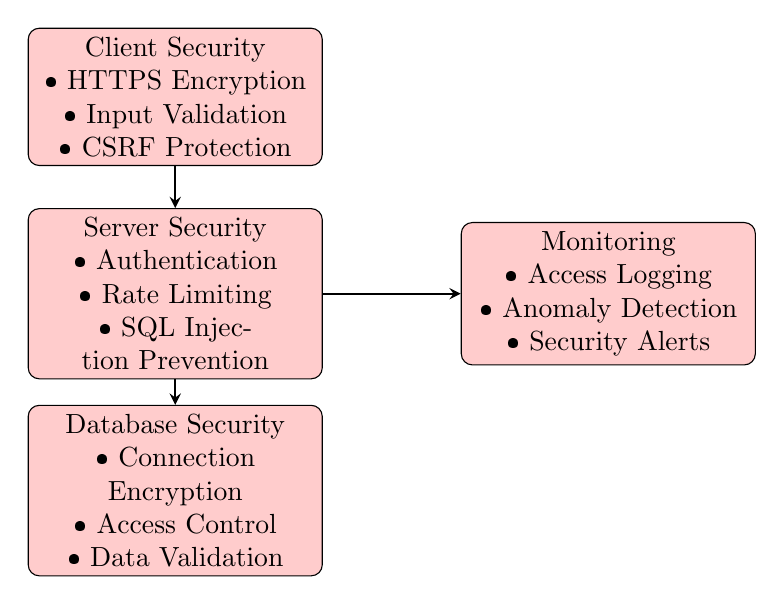
\begin{tikzpicture}[
    node distance=2.5cm,
    security/.style={rectangle, draw, fill=red!20, text width=3.5cm, text centered, rounded corners, minimum height=1.5cm}
]

% Security layers
\node[security] (client) {Client Security\\• HTTPS Encryption\\• Input Validation\\• CSRF Protection};

\node[security, below of=client] (server) {Server Security\\• Authentication\\• Rate Limiting\\• SQL Injection Prevention};

\node[security, below of=server] (database) {Database Security\\• Connection Encryption\\• Access Control\\• Data Validation};

\node[security, right of=server, xshift=3cm] (monitoring) {Monitoring\\• Access Logging\\• Anomaly Detection\\• Security Alerts};

% Arrows showing security flow
\draw[->, >=stealth, thick] (client) -- (server);
\draw[->, >=stealth, thick] (server) -- (database);
\draw[->, >=stealth, thick] (server) -- (monitoring);

\end{tikzpicture}
\caption{Multi-layered security architecture protecting different system components}
\label{fig:security-architecture}
\end{figure}

The security measures illustrated in Figure~\ref{fig:security-architecture} provide comprehensive protection across all system layers, ensuring data integrity and user privacy.

\section{Deployment Architecture}

The deployment strategy utilizes containerization and cloud services for scalability and reliability. Figure~\ref{fig:deployment-architecture} shows the production deployment setup.

\begin{figure}[!htbp]
\centering
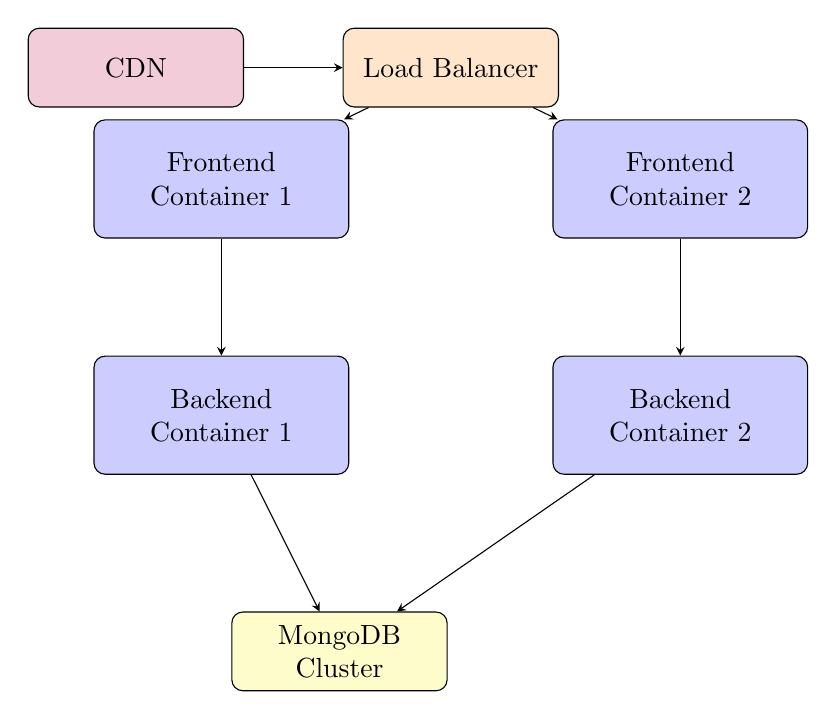
\begin{tikzpicture}[
    node distance=2cm,
    container/.style={rectangle, draw, fill=blue!20, text width=3cm, text centered, rounded corners, minimum height=1.5cm},
    service/.style={rectangle, draw, fill=green!20, text width=2.5cm, text centered, rounded corners, minimum height=1cm}
]

% Load Balancer
\node[service, fill=orange!20] (lb) {Load Balancer};

% Application containers
\node[container, below left of=lb, xshift=-1.5cm] (app1) {Frontend\\Container 1};
\node[container, below right of=lb, xshift=1.5cm] (app2) {Frontend\\Container 2};

% Backend containers
\node[container, below of=app1, yshift=-1cm] (api1) {Backend\\Container 1};
\node[container, below of=app2, yshift=-1cm] (api2) {Backend\\Container 2};

% Database cluster
\node[service, below of=api1, xshift=1.5cm, yshift=-1cm, fill=yellow!20] (db) {MongoDB\\Cluster};

% CDN
\node[service, left of=lb, xshift=-2cm, fill=purple!20] (cdn) {CDN};

% Arrows
\draw[->, >=stealth] (cdn) -- (lb);
\draw[->, >=stealth] (lb) -- (app1);
\draw[->, >=stealth] (lb) -- (app2);
\draw[->, >=stealth] (app1) -- (api1);
\draw[->, >=stealth] (app2) -- (api2);
\draw[->, >=stealth] (api1) -- (db);
\draw[->, >=stealth] (api2) -- (db);

\end{tikzpicture}
\caption{Production deployment architecture with load balancing and container orchestration}
\label{fig:deployment-architecture}
\end{figure}

The deployment architecture in Figure~\ref{fig:deployment-architecture} ensures high availability and scalability through load balancing, containerization, and distributed database architecture.

\section{Performance Optimization}

Performance optimization strategies are implemented at multiple levels of the system. The optimization approach is summarized in Figure~\ref{fig:performance-optimization}.

\begin{figure}[H]
\centering
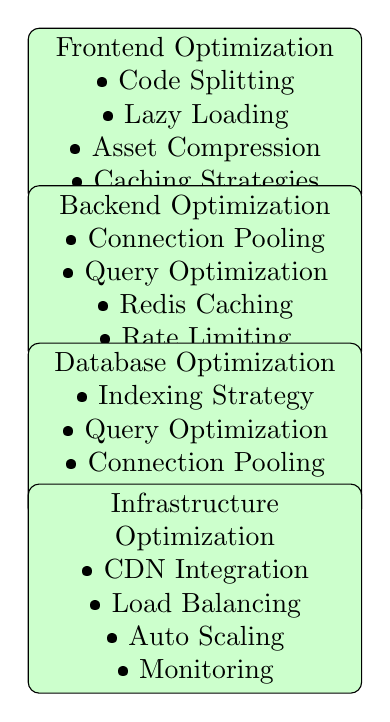
\begin{tikzpicture}[
    node distance=2cm,
    opt/.style={rectangle, draw, fill=green!20, text width=4cm, text centered, rounded corners, minimum height=1.2cm}
]

% Frontend optimizations
\node[opt] (frontend) {Frontend Optimization\\• Code Splitting\\• Lazy Loading\\• Asset Compression\\• Caching Strategies};

% Backend optimizations
\node[opt, below of=frontend] (backend) {Backend Optimization\\• Connection Pooling\\• Query Optimization\\• Redis Caching\\• Rate Limiting};

% Database optimizations
\node[opt, below of=backend] (database) {Database Optimization\\• Indexing Strategy\\• Query Optimization\\• Connection Pooling\\• Replica Sets};

% Infrastructure optimizations
\node[opt, below of=database] (infra) {Infrastructure Optimization\\• CDN Integration\\• Load Balancing\\• Auto Scaling\\• Monitoring};

\end{tikzpicture}
\caption{Comprehensive performance optimization strategies across all system layers}
\label{fig:performance-optimization}
\end{figure}

The performance optimization strategies shown in Figure~\ref{fig:performance-optimization} ensure optimal response times and efficient resource utilization across the entire system.

\section{Conclusion}

The Ziplink system design implements a robust, scalable architecture that efficiently handles URL shortening operations while providing comprehensive analytics and user management features. The modular design with proper figure placement ensures maintainability and extensibility for future enhancements.

Key architectural benefits include:
\begin{itemize}
    \item Scalable three-tier architecture
    \item Modern frontend with React and Vite
    \item RESTful API design with Express.js
    \item Efficient MongoDB database schema
    \item Comprehensive security measures
    \item Performance optimization at all layers
\end{itemize}

This design document serves as a comprehensive guide for developers and stakeholders, with all diagrams strategically placed near their corresponding explanatory text for optimal readability and understanding.

\end{document}